
\documentclass[twoside,twocolumn]{article}
\usepackage{stackengine}
\usepackage{blindtext} 
\usepackage{amsmath}
\usepackage[sc]{mathpazo} 
\usepackage[T1]{fontenc} 
\linespread{1.05} 
\usepackage{microtype} 
\usepackage{amssymb}
\usepackage[italian]{babel} 
\usepackage{tikz}
\usepackage[hmarginratio=1:1,top=32mm,columnsep=20pt]{geometry} 
\usepackage[hang, small,labelfont=bf,up,textfont=it,up]{caption} 
\usepackage{booktabs} 
\usepackage{tocbibind}
\newtheorem{theorem}{Teorema}
\newtheorem{lemma}{Lemma}
\newcommand{\listofalgorithmes}{\tocfile{\listalgorithmcfname}{loa}}
\usepackage{lettrine} 
\usepackage{graphicx} 
\usepackage{enumitem} 
\setlist[itemize]{noitemsep} 
\usetikzlibrary{shapes.misc, positioning}
\usepackage{abstract} 
\renewcommand{\abstractnamefont}{\normalfont\bfseries}
\renewcommand{\abstracttextfont}{\normalfont\small\itshape} 
\usepackage{titlesec} 
\renewcommand\thesection{\Roman{section}} 
\renewcommand\thesubsection{\roman{subsection}} 
\newcommand{\notimplies}{%
	\mathrel{{\ooalign{\hidewidth$\not\phantom{=}$\hidewidth\cr$\implies$}}}}
\titleformat{\section}[block]{\large\scshape\centering}{\thesection.}{1em}{} 
\titleformat{\subsection}[block]{\large}{\thesubsection.}{1em}{}
\usepackage{fancyhdr} 
\pagestyle{fancy} 
\fancyhead{} 
\fancyfoot{} 
\fancyhead[C]{BetaReg $\bullet$ Applied Statistic and Data Analysis} % Custom header text
\fancyfoot[RO,LE]{\thepage} 

\usetikzlibrary{positioning}

\newcommand{\LivelloReale}{Livello reale}
\newcommand{\LivelloAstratto}{Livello astratto }
\newcommand{\qzero}{$q_0$}
\newcommand{\quno}{$q_1$}
\newcommand{\qdue}{$q_2$}
\newcommand{\qtre}{$q_3$}
\newcommand{\qzerohat}{$\hat{q_0}$}
\newcommand{\qunohat}{$\hat{q_1}$}
\newcommand{\yslant}{0.5}
\newcommand{\xslant}{-0.6}

\usepackage{titling}

\usepackage{hyperref} 

\usepackage{algorithm2e} %for psuedo code
 \SetKwProg{Fn}{function}{}{end-function}
  \SetKwProg{Try}{try}{}{}
  \SetKwProg{Catch}{catch}{}{end}
 \RestyleAlgo{boxed}
%\usepackage[lmargin=3.81cm,tmargin=2.54cm,rmargin=2.54cm,bmargin=2.52cm]{geometry}

\def\rlwd{.4pt}
\def\rlht{1.1pt}
\def\shatvrule{\rule{\rlwd}{\rlht}}
\def\shat#1{%
	\setbox0=\hbox{$#1$}%
	\stackon[0pt]{\stackon[1pt]{\ensuremath{#1}}{%
			\shatvrule\kern\wd0\kern-\rlwd\kern-\rlwd\shatvrule}}%
	{\rule{\wd0}{\rlwd}}%
}

\setlength{\droptitle}{-4\baselineskip} 

\pretitle{\begin{center}\Huge\bfseries} 
	\posttitle{\end{center}} 
\title{BetaReg: pacchetto R} 
\author{
	\textsc{Marta Rotari - Idriss Riouak} \\[1ex] 
	\normalsize Università degli studi di Udine \\ 
	\normalsize Dipartimento di matematica e informatica \\ 
	\normalsize Applied Statistic and Data Analysis\\
	\normalsize \href{mailto:idriss.riouak@spes.uniud.it}{idriss.riouak@spes.uniud.it} 
	\normalsize \href{mailto:marta.rotari@spes.uniud.it}{marta.rotari@spes.uniud.it} 
}
\date{\today} 
\renewcommand{\maketitlehookd}{%
	\begin{abstract}
		\noindent  La regressione è un metodo statistico che permette l'analisi delle relazioni che intercorrono tra due variabili che possono assumere valori nel continuo o nel discreto. Lo scopo di questa relazione è quello di studiare e analizzare un modello di regressione nel quale il dominio delle variabili di risposta possono assumere valori nell'intervallo limitato $(0,1)$.
		Il modello analizzato è chiamato modello di regressione con variabili di risposta Beta, introdotto per la prima volta nel 2004 da Cribari-Neto e Ferrari \cite{2004}. In particolare andremo ad analizzare l'implementazione in \emph{R} del modello, evidenziandone i pregi e difetti.
	\end{abstract}
}


\begin{document}
	

	\maketitle
	
	\section{Introduzione}
	Un modello di regressione è un modello statistico, il cui scopo è sia quello di studiare ed analizzare le relazioni tra una una variabile \emph{dipendente}, detta variabile di risposta, e una o più variabili \emph{indipendenti}, dette variabili esplicative, che di effettuare predizioni dato un nuovo valore per la variabile esplicativa.
	
	Il \emph{modello di regressione lineare semplice} ha la seguente forma
	$$ y_i=\alpha + \beta x_i + \varepsilon_i $$
	dove la componente casuale $\varepsilon_i$ è normalmente distribuita con media zero e varianza $\sigma^2$.
	
	Prima dell'avvento del modello di regressione con variabili Beta, per effettuare un'analisi di regressione in cui la variabile di risposta (v.r.) $y$ assumeva valori in (0,1), era consuetudine effettuare delle trasformazioni di $y$. Dunque si considerava $\tilde{y}=log(\frac{y}{1-y})$ alla quale veniva applicato il modello di regressione lineare semplice. Tale approccio presentava le seguenti problematiche:
	\begin{enumerate}[label=\Roman*]
		\item Disugaglianza di Jensen: ovvero i parametri dovevano essere interpretati rispetto il valore atteso di $\tilde{y}$ anziché rispetto quello di $y$.
		\item Eteroschedasticità: la varianza aumentava all'avvicinarsi della media e decresceva spostandosi versoi limiti dell'intervallo.
		\item Asimmetria: in generale la distribuzione di tassi e di proporzioni è asimmetrica e dunque la stima degli intervalli per il test dell'ipotesi basate su approssimazioni Gaussiane potrebbero essere imprecise per campioni di piccole dimensioni.
	\end{enumerate}
	Nel 2004, Cribari-Neto e Ferrari, con l'articolo \emph{``Beta Regression for Modelling Rates and Proportions"} \cite{2004}, descrivono come il modello di regressione con variabili Beta sia il migliore per trattare proporzioni e tassi. Successivamente nel 2016, nell'articolo \emph{``Beta Regression in R''} \cite{CNF}, i due autori forniscono un'implementazione in R di tale modello.
	
	\section{Beta distribuzione}
	Come già anticipato, il modello di regressione con variabili Beta, d'ora in avanti BetaReg, si presta perfettamente per modellare situazioni in cui la variabile di risposta $y$ assuma valori nell'intervallo aperto (0,1)\footnote{Si noti che se la variabile $y$ dovesse assumere valori nell'intervallo $(a,b)$, dove $a < b$ e sia $a$ che $b$ sono valori noti, allora è possibile modellare $\frac{y-a}{b-a}$ al posto di $y$. Mentre se la variabile $y$ dovesse assumere come valori in [0,1], una possibile trasformazione potrebbe essere $\frac{y\cdot (n-1) \cdot 0.5}{n}$ dove $n$ è la grandezza del campione.}. 
	
	BetaReg è basato su un'alternativa parametrizzazione della funzione di densità della distribuzione beta;
	la funzione di densità di una variabile casuale (v.c.) beta è data nel seguente modo
	$$f(y;p,q)=\frac{\Gamma(p+q)}{\Gamma(p)\Gamma(q)}y^{p-1}(1-y)^{q-1},\ \ \ \ 0 <y<1$$ 
	Dove $p>0$ e $q>0$ e $\Gamma(\cdot)$ è la funzione gamma. 
	
	\emph{Ferrari e Cribari-Neto}, hanno proposto una parametrizzazione differente:
	$$ f(y,\mu,\phi)=\frac{\Gamma{\phi}}{\Gamma(\mu\phi)\Gamma((1-\mu)\phi)}y^{\mu\phi^{-1}}(1-y)^{(1-\mu)\phi-1} $$
	con 
	\begin{align*}
	\mu&=\frac{p}{p+q} \ , & \phi=p+q
	\end{align*}
	dove $0<\mu<1$, $\phi >0 $ e $0<y<1$. 
		\begin{figure}[h]
		\hspace*{-0.5cm}
		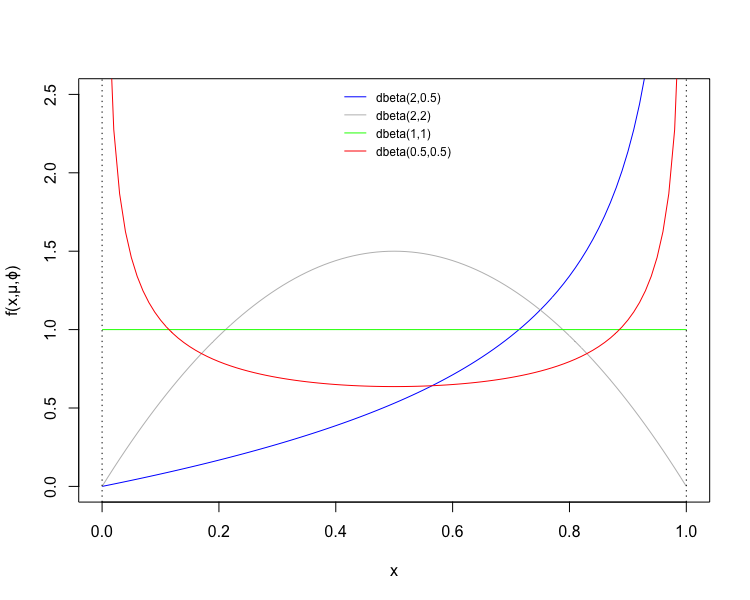
\includegraphics[scale=.3]{Beta}
		\caption{Rappresentazione grafica della distribuzione Beta, utilizzando il comando R: \emph{dbeta}.}
	\end{figure}
	
	
	
	Denoteremo con $y \sim \mathbb{\mathcal{B}}(\mu,\phi)$ se  la v.c. $y$ segue una beta distribuzione con parametri $\mu$ e $\phi$. Si noti che $p=\mu\phi$ e $q=\phi(1-\mu)$, da cui segue che $E(y)=\mu$ e che $VAR(y)=\frac{V(\mu)}{1+\phi}=\frac{\mu(1-\mu)}{1+\phi}$. 
	
	Il parametro $\phi$ è anche chiamato \emph{parametro di precisione}, in quanto  per un fissato $\mu$, all'aumentare di $\phi$ diminuisce il valore della varianza.

\section{Il modello di regressione Beta}
Sia $y_1, y_2, ... ,y_n$ un campione casuale tale che $	\forall_{i=1}^n: y_i \sim \mathbb{\mathcal{B}}(\mu_i, \phi)$. Il modello di regessione Beta è definito nel seguente modo
$$ g(\mu_i)=x_i^t\beta=\eta_i$$
dove $\beta=(\beta_1, \beta_2, ..., \beta_k)^t$, con $k<n$, è un vettore $k \times 1$, $x_i=(x_{i1}, x_{i2},...,x_{ik})^t$ è un vettore di $k$ variabili esplicative mentre $\eta_i=\beta_1x_{i1}...\beta_kx_{ik}$\footnote{Per convenzione $x_{i1}=1$. In tal modo ogni modello ha l'intercetta (null-model) \cite{PV}. } è un predittore lineare. Infine $g(\cdot):(0,1)\rightarrow\mathbb{R} \in \mathcal{C}^2$ è una funzione  di collegamento avente derivata seconda costante.

	
\newpage
\tableofcontents
\listofalgorithmes

		\begin{thebibliography}{99} 
	\bibitem{2004} \textbf{Beta Regression for Modelling Rates and Proportions.}, Ferrari SLP, Cribari-Neto Francisco (2004).  Journal of Applied Statistics, 31(7), 799–815.
	\bibitem{CNF} \textbf{Beta Regression in R}, Francisco Cribari-Neto, Achim Zeileis.\\
	\bibitem{PV} \textbf{Towards multiple linear regression and logistic regression}, Paolo Vidoni, 2017-2018. Lecture 5. Applied Statistics and Data Analysis.
	\end{thebibliography}

\end{document}